The complexity of a \ac{LBA} increases with the complexity of the system it has
to work with.
Consider a load balancing algorithm that computes the target worker for a task,
where the size of the tasks are equal, the workers have the same capabilities
and the number of overall tasks is known.
Such an algorithm is not of complexity.
In fact, it can be implemented by a simple mathematical equation:
\begin{equation}
    i = j \% |W|
\end{equation}
Where $i$ is the number of the worker instance in set $W$ that will be assigned
with the task number $j$.
Though, such an environment is unlikely.

In todays systems, the size of a task cannot be predicted.
The capabilities of a worker instance may be known, but as tasks come in and are
assigned to workers, an algorithm has to implement some book-keeping to know
which worker has the least load at a given point in time.
This is not complex, though having only one load balancer in a large ecosystem
is highly unlikely, as it would be a single point of failure.
Instead, multiple load balancers are used.
Because of this, some synchronization method between the book-keeping of each
load balancer must be introduced to ensure the best distribution of tasks.

If worker instance $W_1$ has the least load at time $t_1$, the load balancer
$L_1$ might assign a number of tasks to it in $t_2$.
After that, $L_1$ must notify $L_2$ about the new load on $W_1$, which it does
in $t_3$.
In the meantime, load balancer $L_2$ might need to assign another set of tasks,
which it assignes to $W_1$ in $t_2$, because it does not know yet that $W_1$
isn't the least loaded worker anymore.
This causes $W_1$ to become overloaded in $t_3$.

\subsection{Random load balancing}

A cheap load balancing strategy is randomizing the target.
\begin{equation}
    i = rand() \% |W|
\end{equation}
Which has several advantages over other approaches:
\begin{itemize}
    \item Simplicity
    \item Few edge cases
    \item Easy failover
    \item Works distributed
\end{itemize} % TODO: cite http://www.codemesh.io/codemesh/tyler-mcmullen ?
Although, distributing load randomly does not guarantee the best distributing
over a given set of notes.
It is even possible that a small set of workers are assigned
with a huge number of tasks while other workers only handle a very small number
of tasks, resulting in a high load on some machines while others idle.

The desireable state is that each machine has the same workload, resulting in a
perfect distribution of load over all machines.
With an algorithm randomly assigning work to workers, the possibility exists
that the system ends up in an unbalanced state.
Though this is very unlikely, we can do better.

\subsection{\ac{JSQ}}

Another known load balancing algorithm is \ac{JSQ}.
With this algorithm, the load balancing mechanism implements some book-keeping
mechanism how many jobs are in the queues of the worker instances and selects
the instance with the shortest queue for a new task.
This algorithm can result in a ``herd effect'' in distributed environments,
where a subset of machines is either underutilized or overloaded with tasks.
That is likely, if the load balancing instance(s) has old information on the
utilization of the nodes as described in \cite{inpSLoadInfo}.

A surprisingly good optimization is the combination of the two algorithms
described above.
\begin{equation}
    \begin{aligned}
        x &= rand() \% |I| \\
        y &= rand() \% |I| \\
        i &= \begin{cases}
            x & \text{if } load(W_x) =< load(W_y)\\
            y & \text{if } load(W_x) > load(W_y)\\
        \end{cases}
    \end{aligned}
    \label{eq:randjsq}
\end{equation}
If we combine these algorithms, so we select two worker instances randomly and
now apply \ac{JSQ} on this new set of worker instances (see \ref{eq:randjsq}),
we get better distribution, as stated in \cite{powerOfTwoInRLB}.

\subsection{Example load balancing output}

The load balancing algorithms ``Random'', ``Roundrobin'', ``\ac{JSQ}'' and
``select-random-\ac{JSQ}'' were implemented in the Rust programming language to
visualize their behaviour.
Figure \ref{fig:algo:use} visualizes the results of the load balancing
algorithms applied to a set of data.
The input values were five worker machines and $10,000$ tasks.
The figure shows how much work each worker must handle.
A perfect distribution would result in each worker handling $20\%$ of the tasks.

% TODO: Fix numbering
\begin{figure}
	\centering
	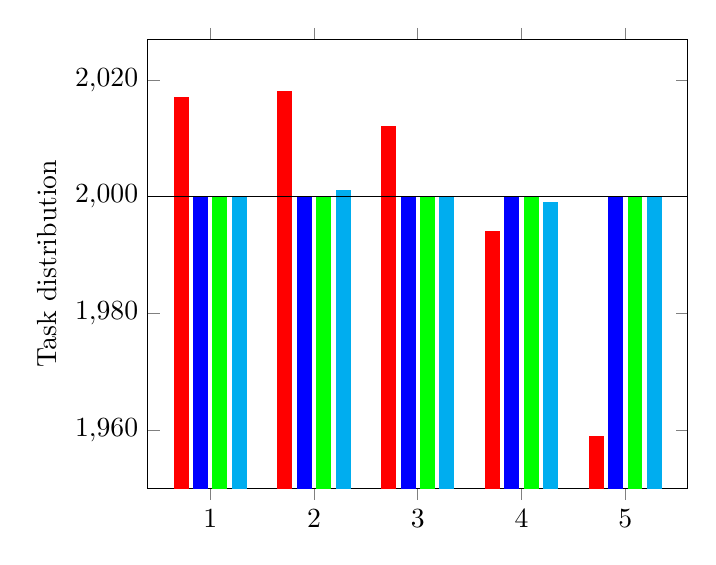
\begin{tikzpicture}
		\begin{axis}[
			ybar,
			enlargelimits=0.15,
			ylabel={Task distribution},
			symbolic x coords={0,1,2,3,4,5,6},
			xtick=data,
			nodes near coords align={vertical},
			bar width=5pt,
			]
			\addplot+[color=red] % Random
			coordinates {(1,2017) (2,2018) (3,2012) (4,1994) (5,1959)};

			\addplot+[color=blue] % Roundrobin
			coordinates {(1,2000) (2,2000) (3,2000) (4,2000) (5,2000)};

			\addplot+[color=green] % JSQ
			coordinates {(1,2000) (2,2000) (3,2000) (4,2000) (5,2000)};

			\addplot+[color=cyan] % select-random-JSQ
			coordinates {(1,2000) (2,2001) (3,2000) (4,1999) (5,2000)};

			\addplot[black,line legend,sharp plot,update limits=false]
				coordinates {(0,2000) (6,2000)};
		\end{axis}
	\end{tikzpicture}
	\label{fig:algo:use}
	\caption{Task distribution}
\end{figure}

\begin{figure}
	\centering
	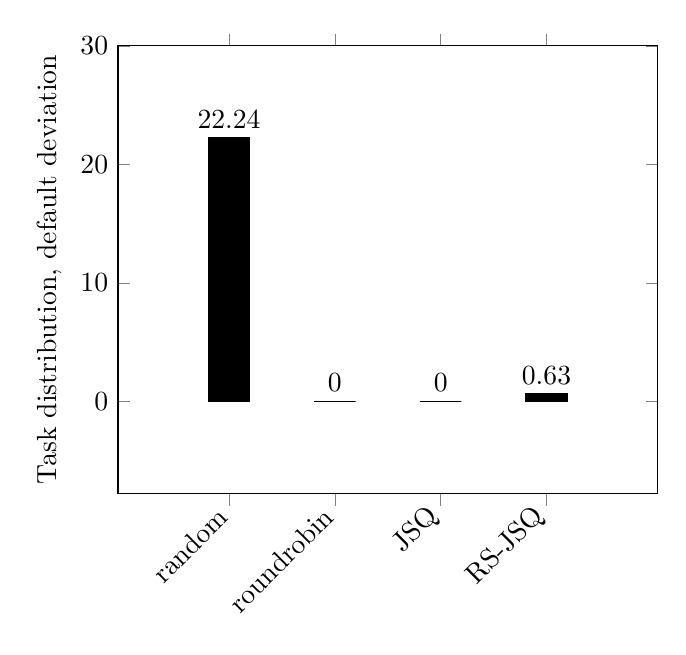
\begin{tikzpicture}
		\begin{axis}[
			ybar,
			enlargelimits=0.35,
			ylabel={Task distribution, default deviation},
			symbolic x coords={random,roundrobin,JSQ,RS-JSQ},
			xtick=data,
			nodes near coords,
			nodes near coords align={vertical},
			x tick label style={rotate=45,anchor=east},
			bar width=15pt,
			]

			\addplot+[color=black] coordinates
			{(random,22.24) (roundrobin,0) (JSQ,0) (RS-JSQ,0.632)};

		\end{axis}
	\end{tikzpicture}
	\label{fig:algo:use:defdev}
	\caption{Load distribution, default deviation}
\end{figure}

The figure in \ref{fig:algo:use} does not visualize, though what the
\emph{load} values on each of these instances are, as this value is hardly
predictable.
The figure in \ref{fig:algo:load} visualized the load distribution which results
from the above distribution of tasks.
The load for each task was a random number ranging from $1$ to $4$, where $4$ is
a high load requirement.

\begin{figure}
	\centering
	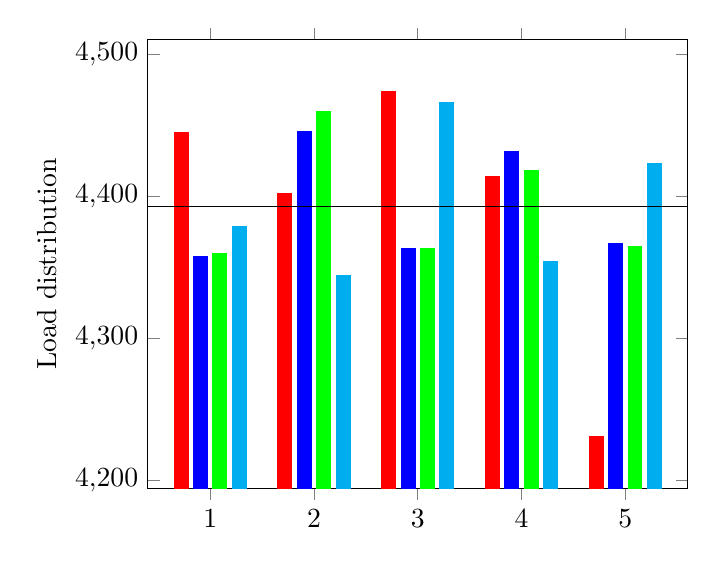
\begin{tikzpicture}
		\begin{axis}[
			ybar,
			enlargelimits=0.15,
			ylabel={Load distribution},
			symbolic x coords={0,1,2,3,4,5,6},
			xtick=data,
			nodes near coords align={vertical},
			bar width=5pt,
			]

			\addplot+[color=red] % Random
			coordinates {(1,4445) (2,4402) (3,4474) (4,4414) (5,4231)};

			\addplot+[color=blue] % Roundrobin
			coordinates {(1,4358) (2,4446) (3,4363) (4,4432) (5,4367)};

			\addplot+[color=green] % JSQ
			coordinates {(1,4360) (2,4460) (3,4363) (4,4418) (5,4365)};

			\addplot+[color=cyan] % RS-JSQ
			coordinates {(1,4379) (2,4344) (3,4466) (4,4354) (5,4423)};

			\addplot[black,line legend,sharp plot,update limits=false]
				coordinates {(0,4393) (6,4393)};
		\end{axis}
	\end{tikzpicture}
	\label{fig:algo:load}
	\caption{Load distribution}
\end{figure}

\begin{figure}
	\centering
	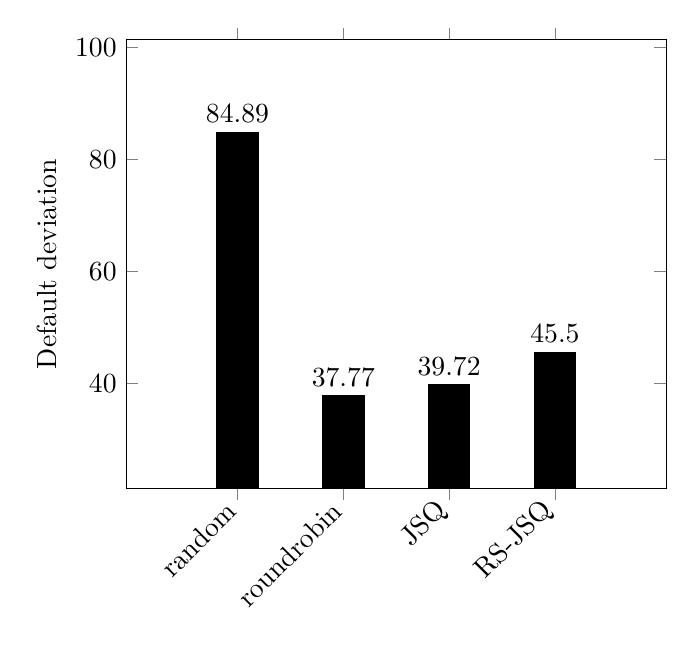
\begin{tikzpicture}
		\begin{axis}[
			ybar,
			enlargelimits=0.35,
			ylabel={Default deviation},
			symbolic x coords={random,roundrobin,JSQ,RS-JSQ},
			xtick=data,
			nodes near coords,
			nodes near coords align={vertical},
			x tick label style={rotate=45,anchor=east},
			bar width=15pt,
			]

			\addplot+[color=black] coordinates
				{(random,84.889)
				(roundrobin,37.765)
				(JSQ,39.716)
				(RS-JSQ,45.497)};

		\end{axis}
	\end{tikzpicture}
	\label{fig:algo:load:defdev}
	\caption{Load distribution, default deviation}
\end{figure}

% vim: set ts=4 sw=4 tw=0 noet :
